% Define document class. Options: article, report, book, ...
\documentclass{report}

% Include preamble.tex
% Needed to add contents to toc without hyperlink
\let\origcontentsline\contentsline
\let\origaddtocontents\addtocontents

% Include packages
\usepackage[utf8]{inputenc}
% caption is used to jump to top of image, table and not to caption.
\usepackage{amsmath, amsfonts, amsthm, graphicx, tabularray, adjustbox, geometry, lipsum, caption, setspace, fancyvrb, fancyhdr, lastpage, etoolbox, xcolor, tikz, tcolorbox, siunitx, tocloft, hyperref, float, pdfpages}
\usepackage[Lenny]{fncychap} %Options: Sonny, Lenny, Glenn, Conny, Rejne, Bjarne, Bjornstrup
\usepackage[acronym]{glossaries-extra}
\usepackage[hyperref=true, backref=true, backend=biber, style=apa, sorting=nyt]{biblatex}

% Set page margins (package: geometry)
\newgeometry{
    top=3cm,
    bottom=2.5cm,
    outer=4cm,
    inner=4.5cm
}

% Set title of pdf and color of internal and external links (package: hyperref)
\hypersetup{
    linktoc=all,
    colorlinks=true,
    linkcolor=black,
    citecolor=black,
    urlcolor=blue,
    pdftitle={Bachelor Thesis}
}

% Needed so that hyperref also works in combination with \appendix
\renewcommand{\theHchapter}{\thepart.\thechapter}

% Set pagestyle of the first page of a new chapter to chapterstart (package: etoolbox)
\patchcmd{\chapter}{plain}{chapterstart}{}{}
% Declare chapterstart and plain pagestyle to have no line, no headers and no footers (package: fancyhdr)
\fancypagestyle{plain}{%
  \renewcommand{\headrulewidth}{0pt} % clear rules
  \fancyhf{} % Clear all header and footer fields.
}
\fancypagestyle{chapterstart}{%
  \renewcommand{\headrulewidth}{0pt} % clear rules
  \fancyhf{} % Clear all header and footer fields.
}

% Set default pagestyle to fancy and declare headers and footers. (package: fancyhdr)
\pagestyle{fancy}
\renewcommand{\chaptermark}[1]{\markboth{#1}{}}
\renewcommand{\sectionmark}[1]{\markright{#1}{}}
\cfoot{} % clear default page number in center
% Use the following for alternating headers if doucment is printed
%\fancyhead{} % clear all header fields
%\fancyhead[LO,RE]{\nouppercase\leftmark}
%\fancyhead[RO,LE]{\thepage}
% Use following for static headers if document only used as pdf
\lhead{\nouppercase\leftmark}
\rhead{\thepage}
%\rfoot{Page \thepage\ of \pageref{LastPage}}

% Format chapter title (package: fancychap)
\ChNameUpperCase
%\ChNumVar{\fontsize{40}{42}\usefont{OT1}{ptm}{m}{n}\selectfont}
\ChTitleVar{\huge\sc}

% Increase space between text by 50 % (package: setspace)
\onehalfspacing 

% Increase space between table rows by 0.3 em (package: tabularray)
\SetTblrInner{rowsep=0.3em}

% Remove indentation in list of figures and list of tables
\makeatletter
\renewcommand*\l@figure{\@dottedtocline{1}{0em}{2.3em}} % Default: 1.5em/2.3em
\let\l@table\l@figure
\makeatother

% Define acronym style and create glossary (package: glossaries-extra)
\setabbreviationstyle[acronym]{long-short}
\makeglossaries

% Add bib resource and configure blibliography (package: biblatex)
\addbibresource{ref.bib}
\DefineBibliographyStrings{english}{%
    backrefpage  = {\lowercase{s}ee p.}, % for single page number
    backrefpages = {\lowercase{s}ee pp.} % for multiple page numbers
}
\newcommand{\apacite}[1]{(\cite{#1})}
\DeclareBibliographyAlias{artwork}{online} % use online entry type for artwork entries

% Add commands for adding list of equations (package: tocloft)
\newcommand{\cftloetitlefont}{} % new command which allows to format title font of list of equations
\newcommand{\listequationsnamedefaultformat}{List of Equations}
\newcommand{\listequationsname}{\cftloetitlefont{\listequationsnamedefaultformat}}
\newlistof{myequations}{equ}{\listequationsname}
\newcommand{\myequations}[1]{\addcontentsline{equ}{myequations}{\protect\numberline{\theequation}#1}\par}

% Reformat headings of listings (package: tocloft)
\renewcommand\cfttoctitlefont{\huge\sc} % toc
\renewcommand\cftloftitlefont{\huge\sc} % list of figures
\renewcommand\cftlottitlefont{\huge\sc} % list of tables
\renewcommand\cftloetitlefont{\huge\sc} % list of equations

% Add auto indentation to captions (package: caption)
\captionsetup{format=hang}

% Include acronyms and glossary declarations
\newacronym{sota}{SotA}{state-of-the-art}
\newacronym{hslu}{HSLU}{Lucerne University of Applied Sciences and Arts}
\newacronym{cnn}{CNN}{Convolutional Neural Network}
%\newacronym{}{}{}
\newglossaryentry{latex}
{
    name=latex,
    description={Is a markup language specially suited 
    for scientific documents}
}

\newglossaryentry{maths}
{
    name=mathematics,
    description={Mathematics is what mathematicians do}
}

% Start of document content
\pagenumbering{roman}
\begin{document}

\thispagestyle{empty}
\begin{figure}[ht]
    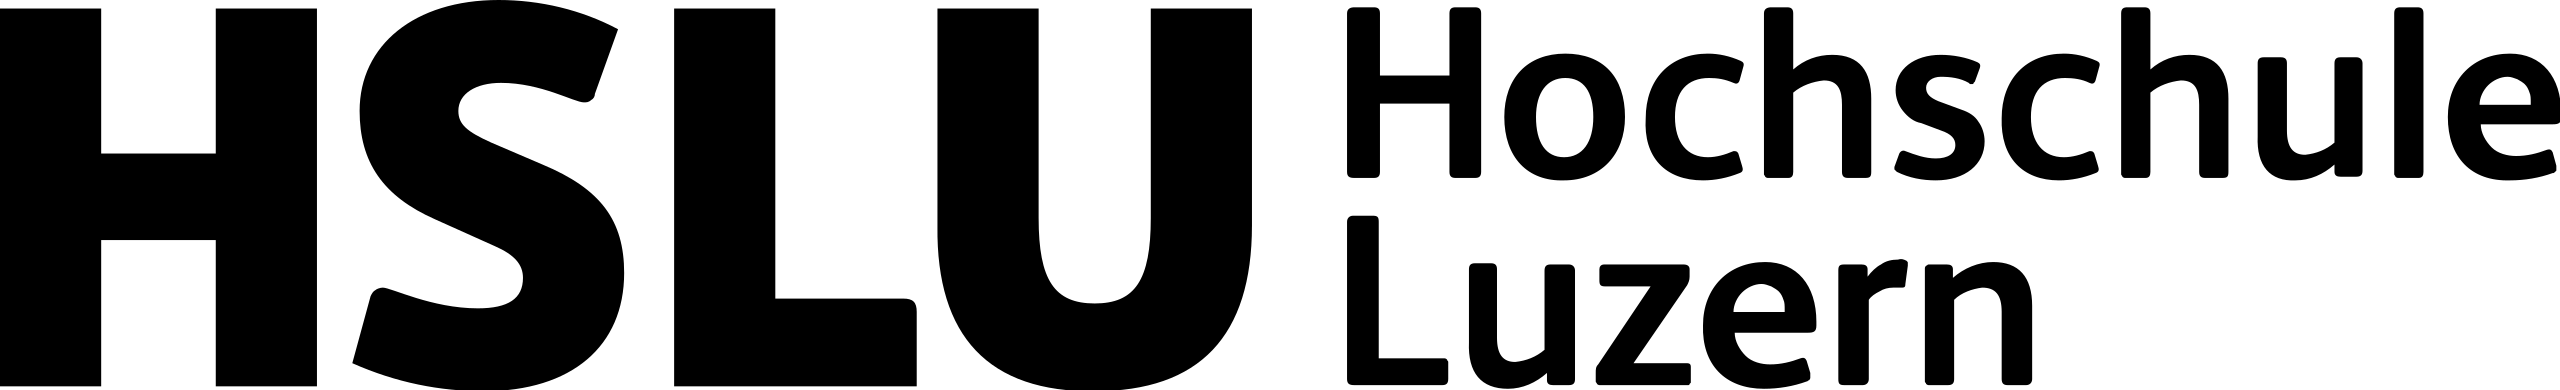
\includegraphics[width=20em,height=\textheight,keepaspectratio]{images/hslu_2022_logo.png}
\end{figure}
\vspace*{9em}

\noindent\begin{center}
\huge{\textbf{Machine Learning for the Prediction of Refractive Surprise after Cataract Surgery}}\\
\vspace*{3em}

\Large{Bachelor Thesis}\\
\Large{B.Sc. in Computer Science}\\
\vspace*{4em}

\Large{by}\\
\Large{\textbf{Your Name}}\\
\Large{03\textsuperscript{th} of January 2023}\\
\vspace*{\fill}

\large{Advisors:\\Dr. John Doe, Dr. sc. ETH Max Mustermann}
\end{center}
\thispagestyle{empty}
\vspace*{\fill}
\begin{center}
    \copyright\ 2023\\
    Your Name\\
    ALL RIGHTS RESERVED
\end{center}
\chapter*{Declaration}
\chapter*{Abstract}

% Add empty page for double sided print
\newpage 
\thispagestyle{empty}
\ % The empty page
\newpage
\chapter*{Acknowledgements}


\tableofcontents
\thispagestyle{empty}

\chapter*{Demo}
\section*{Cite}
Test cite \apacite{yamauchi_use_2021}.

\section*{Hyperref}
Test Href \href{http://google.ch}{Google}. You can also jump to a chapter or section (see \ref{ch:introduction}). We can also jump to the appendix (see \ref{app:original_project_description}).

\section*{fancyvbr}

\begin{Verbatim}[numbers=left, frame=single]
client = RestClient("localhost:80", "application/json")
students = client.Get("/api/students")
\end{Verbatim}

\section*{color}
Make {\color{red} this} red.

\section*{tcolorbox}
\begin{tcolorbox}
This is a tcolorbox.
\end{tcolorbox}

\section*{Glossary}
The \gls{latex} typesetting markup language is specially suitable 
for documents that include \gls{maths}. 

\section*{Acronym}
This is a \gls{cnn} and the second \gls{cnn}.

\section*{SI units}
\[5 kg m /s^2\]

\[5\ \mathrm{kg}\ \mathrm{m}/\mathrm{s}^2\]

\[5\ \si{kg.m/s^2}\]

\section*{Tables}
\subsection*{Simple Table}
In this thesis you should always use a forward reference for your tables \ref{tab:demo}.
\begin{table}[ht]
\centering
\begin{adjustbox}{max width=\textwidth}
\begin{tblr}{ l|l|l } 
 metric & average & other \\ 
 \hline
 accuracy & 90 \% & 65 \% \\ 
 precision & 81 \% & 70 \% \\
 f1 & 87 \% & 63 \% \\ 
\end{tblr}
\end{adjustbox}
\caption{This is a demo caption for a simple table.}
\label{tab:demo}
\end{table}

The following table \ref{tab:reference_label_prefix} shows which prefix to use for different types of labels.
\begin{table}[ht]
\centering
\begin{adjustbox}{max width=\textwidth}
\begin{tblr}{ l|l l l l l l l }
 Name & Chapter & Section & Subsection & Equation & Figure & Table & Appendix \\
 \hline
 Abbrev. & ch: & sec: & subsec: & eq: & fig: & tab: & app: \\
\end{tblr}
\end{adjustbox}
\caption{Add some letters to the label to recognize what you are referencing.}
\label{tab:reference_label_prefix}
\end{table}


\section*{Figures}
In this thesis you should always use a forward reference for your figures \ref{fig:demo}.
\begin{figure}[ht]
    \centering
    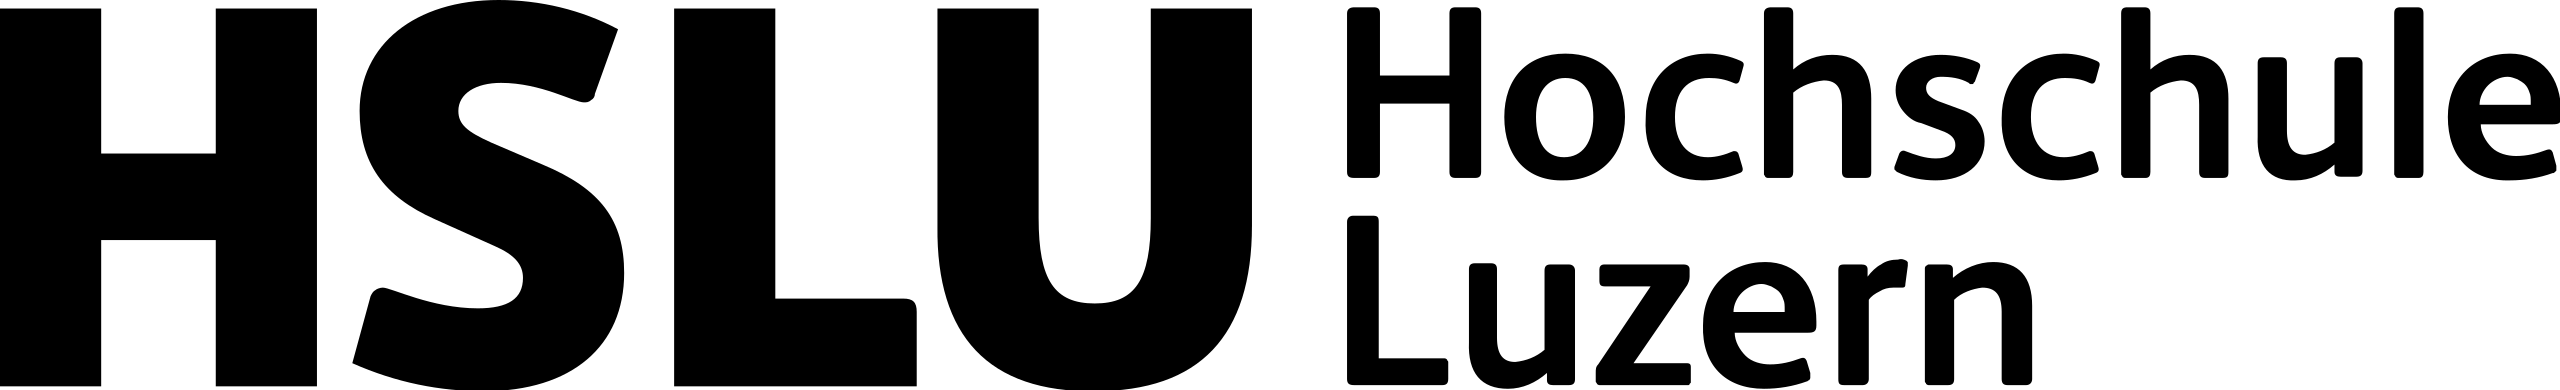
\includegraphics[width=\textwidth,height=\textheight,keepaspectratio]{images/hslu_2022_logo.png}
    \caption{This is a demo caption for a figure.}
    \label{fig:demo}
\end{figure}
\pagenumbering{arabic}
\chapter{Introduction}\label{ch:introduction}
\lipsum[1-10]
\chapter{State-of-the-art}\label{ch:state_of_the_art}
\lipsum[1-10]
\chapter{Concept}\label{ch:concept}
\lipsum[1-10]
\chapter{Methodology}\label{ch:methodology}
\chapter{Realization}\label{ch:realization}
\lipsum[1-10]
\chapter{Evaluation}\label{ch:evaluation}
\chapter{Conclusion}\label{ch:conclusion}
\lipsum[1-10]

\appendix
\part*{Appendix}
\origaddtocontents{toc}{\protect\origcontentsline{part}{Appendix}{}\%}
\chapter{Title}\label{app:a}

\part*{Listings}
\origaddtocontents{toc}{\protect\origcontentsline{part}{Listings}{}\%}
\cleardoublepage
\phantomsection
\addcontentsline{toc}{chapter}{\listfigurename}
\listoffigures

\cleardoublepage
\phantomsection
\addcontentsline{toc}{chapter}{\listtablename}
\listoftables

\printglossary[type=\acronymtype]
\printglossary
\printbibliography[heading=bibintoc, title={Bibliography}]

\end{document}